\documentclass[border=3pt]{standalone}
\usepackage[dvipsnames]{xcolor}
\usepackage{pgfplots}
\usepackage{graphicx}
\renewcommand{\seriesdefault}{\bfdefault}
\pgfplotsset{compat = newest}

 
\begin{document}

 
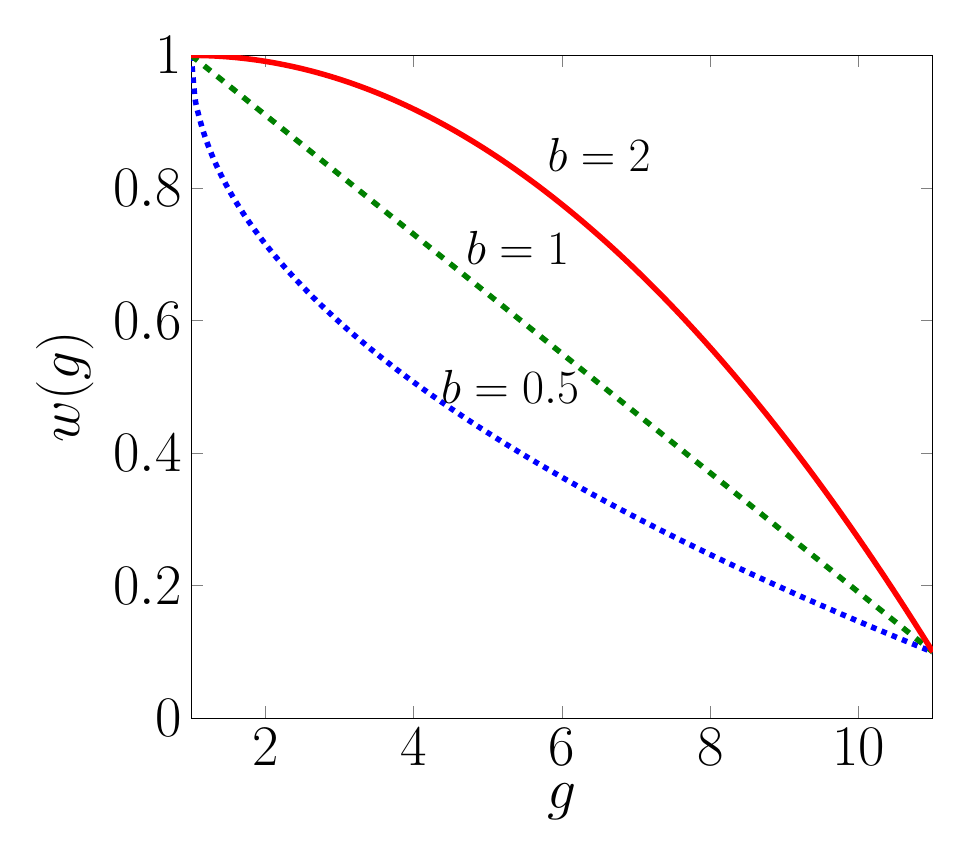
\begin{tikzpicture}
\tikzset{user/.style={circle, inner sep=0pt, minimum size=0.6cm, fill=Black,
    draw=none, text=White, font=\bfseries}}
\begin{axis}[font= \huge,
    xmin = 1, xmax = 11,
    ymin = 0, ymax = 1,
    xlabel = {$g$},
    ylabel = {$w(g)$},width=11cm,height=10cm,
    xtick={0,2, 4, 6,8 ,10},
    ytick={0, 0.2, 0.4 ,0.6,0.8,1}
    ]
    \addplot[line width=2pt,
        domain = 1:11,
        samples = 200,
        smooth,
        dotted,
        blue,
    ] {0.9*(1-((x-1)/10)^0.5)+0.1};
    \addplot[line width=2pt,
        domain = 1:11,
        samples = 200,
        smooth,
        dashed,
        Green,
    ] {0.9*(1-((x-1)/10))+0.1};
    
    \addplot[line width=2pt,
        domain = 1:11,
        samples = 200,
        smooth,
        red,
    ] {(0.9*(1-((x-1)/10)^2)+0.1};

    %\node[font=\small, rotate=90 ] at (6.8,0.2) {$p(k)$};
    %\node[inner sep=0pt] (whitehead) at (9,0.2) {\includegraphics[width=.30\textwidth]{dist_final.png}};
    %\node[font=\small] at (9,0.03) {$k$};
    \node[font= \LARGE] at (6.5,0.85) {$b=2$};
    \node[font= \LARGE] at (5.3,0.5) {$b=0.5$};
    \node[font= \LARGE] at (5.4,0.71) {$b=1$};

    
    
\end{axis}
 
\end{tikzpicture}
 
\end{document}